\subsection{Far Infrared Interferometer and Polarimeter}
The Far InfraRed (FIR) interferometer-polarimeter is a laser diagnostic that employs two different physics principles to measure electron density as well as parallel magnetic field strength. While neither measurement directly informs ion transport, they are critical plasma parameters that are needed to calculate the various terms % which terms?
in the model. I will start by giving a short introduction of the two separate physics principles of the interferometer and then that of the parameter. Then I will describe the FIR hardware as available on MST, and finally, I will describe the analysis and incorporation of raw diagnostic data. 

The FIR interferometer relies on the fact that the index of refraction of the plasma is dependent upon the density of the plasma. In short, one laser beam is passed through the plasma, and then compared with a reference beam that passed through air. The relative phase lag is measured by the interferometer and information about the plasma density is extracted. 

To understand this process in more detail, we can begin with a Fourier representation of the electric field of a generic EM wave:
\begin{align}\label{eqn:fir_wave}
    \vec{E}(\vec{x}, t) &= \frac{1}{(2\pi)^4}\int\vec{E}(\vec{k},\omega)e^{i(\vec{k}\cdot\vec{x}-\omega t)}d^3\vec{k}d\omega 
\end{align}
where $\vec{k}$ is the wave vector, and $\omega$ is the angular frequency. The magnetic field component $\vec{B}(\vec{x},t)$ is similarly described.

In a plasma, an EM wave has to further satisfy the wave equation, as well as Ohm's law, which combines into the following:
\begin{align}
    (\vec{k}\vec{k} - k^2\xtensor{\textbf{1}} + \frac{\omega^2}{c^2}\xtensor{\epsilon})\cdot\vec{B} = 0
\end{align}
where $\xtensor{\epsilon} = (1+\frac{i}{\omega\epsilon_0})$ is the isotropic dielectric constant. Taking the cold plasma approximation of $\xtensor{\epsilon}$ and simplifying the result yields the Appleton-Hartree formula\cite{hutchinson_2002},
%%%Also, you use the first-order approximation lower down, so best to solve the relation to first order here.
\begin{align}
    N^2 &= 1 - \frac{X(1-X)}{1-X-\frac{1}{2}Y^2 \sin^2\theta\pm [(\frac{1}{2}Y^2\sin^2\theta)^2 + (1-X)^2Y^2\cos^2\theta]^{\frac{1}{2}}}
\end{align}
where $N$ is the index of refraction, $X = \frac{\omega_p^2}{\omega^2}$ and $Y = \frac{\Omega}{\omega}$. Considering that the cyclotron frequency $\Omega$ is small compared to the FIR laser frequency $\omega$, then $Y \rightarrow 0$. Taking the zeroth-order approximation\cite{Hutchinson_2002},
\begin{align}
N^2 \approx 1 - \frac{\omega_p^2}{\omega^2}
\end{align}
which is only dependent on $n_e$. Under these conditions, measuring the phase difference between a beam that travels through the plasma and a reference beam traveling through the air will give phase difference
\begin{align}
    \Delta\phi &= \int(k_0 - k_{\text{plasma}})dl \nonumber\\
    &= \frac{\omega}{c}\int(N - 1)dl \nonumber \\
    &= 2.814\times10^{-15}\lambda\int n_e dz 
    &\text{\ [For MST conditions]}
\end{align}
The parameter takes advantage of the 1st order approximation of $N^2$,
\begin{align}
    N^2 = 1 - X \pm XY cos \theta
\end{align}
where the addition refers to the ordinary mode and the subtraction refers to the extraordinary mode. The two modes approximately correspond with right and left handed circularized polarization. Given the differing index of refraction for the two circular polarizations, a phase difference results, leading to an effective rotation of initial polarization referred to as Faraday rotation. The rotation angle is given by,
\begin{align}
    \alpha &= \frac{\Delta \phi}{2}\nonumber\\
    &= \frac{1}{2}(N_+ - N_-)\frac{\omega}{c}z \\
    &\approx \frac{e^2 \lambda^2}{8\pi m^2_e c^3 \epsilon_0}\int n_e \vec{B}\cdot d\vec{l} \nonumber \\
    &= 2.62\times10^{-13}\lambda^2\int n_e{\vec{l}}\vec{B}\cdot d\vec{l} &\text{[For MST conditions]}
\end{align}

\begin{figure}[!htb]
	\centering
	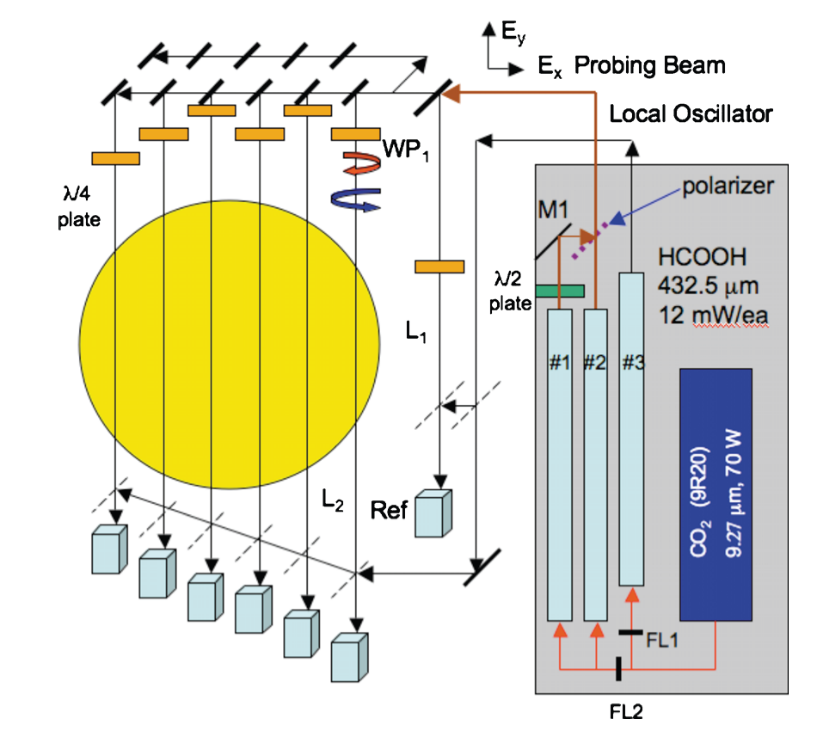
\includegraphics[width = 0.9\linewidth]{./implementation/fir_optics_diagram.PNG}
	\caption[Diagram of FIR optical paths]{Diagram of FIR system optical paths. Lasers marked \#1 and \#2 are orthogonally polarized for polarimetry measurements, and laser \#3 is used as the `local oscillator' necessary for heterodyne phase detection for the interferometry measurements. (Reproduced from E. Parke, et al.\cite{Parke2016})}
    \label{fig:fir_optics_diagram} 
\end{figure}

MST's FIR system consist of a CO$_2$ laser pumping three formic acid cavities in a heterodyne system. The three formic acid cavities are pumped using the same CO$_2$ laser in order to reduce the effects of power fluctuation on the output beam since all three beams are proportional to the pump power. The CO$_2$ pumping laser is a commercially available model with a tunable laser cavity allowing it to be tuned to the FIR pumping frequency. The formic acid laser cavities are custom built and can be tuned independently via motor mounted mirrors. The formic acid lasers convert the ~$10\mu m$ photons from the CO$_2$ laser to ~$432.5\mu m$ (~700GHz) for the probing beams. To facilitate heterodyne detection of phase, the formic acid lasers are further tuned to relative frequencies on the order of 1 MHz. The optical system splits the probing beam into 11 independent measurement chords, as well as separate reference and 'local oscillator' beams paths using thin wire mesh beam splitters. Figure \ref{fig:fir_optics_diagram} provides an illustration of the optical setup. The laser beams, after completing their designated path, are measured with recently installed planar-diode mixers at 6 Mhz. These mixers have high sensitivity and reduced noise floor allowing fluctuation measurements of up to 250 kHz for polarimetry and 600 kHz for interferometry\cite{Parke2016}. 
\begin{figure}[!htb]
	\centering
	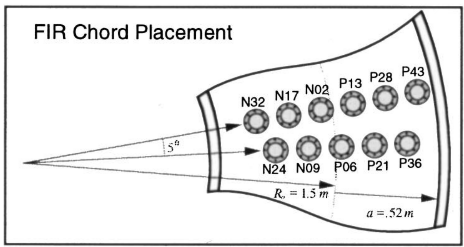
\includegraphics[width = 0.75\linewidth]{./implementation/fir_chords.PNG}

	\caption[Diagram of FIR chord offset]{Diagram of FIR system's 11 viewing chords separated into 2 sets, 5\textdegree\ apart. (Reproduced from N. Lanier, et al.\cite{Lanier2001}}	
	\label{fig:fir_chords}
\end{figure}

The 11 measurement chords are further separated into two sets, about $5\degree$ toroidally separated from each other (see figure \ref{fig:fir_chords}). This has been taken advantages of to make toroidal fluctuation measurements, but for the purpose of the PPCD plasmas investigated in this work, only their radial locations are considered. 

It is pertinent to note that the electron density profile is not determined from a simple inversion of FIR interferometry measurements, but rather incorporated as constraints with other diagnostics measurements in a Grad-Shafranov equilibrium calculation \cite{Anderson2001} as discussed in more detail in section \ref{sec:MSTfit}.